\documentclass[../main.tex]{subfiles}
\graphicspath{{\subfix{../figures/}}}
\begin{document}
\section{Spectrum}
The first step towards simulating the dynamics of the parallel dot system was to calculate the matrix representation of the Liouvillian. This was obtained from the code implementing the PERLind approach mentioned the beginning of this chapter. The code calculates the four jump operators, one for each tunneling process, and then constructs the unitary part of \cref{eq:lind}. Finally, the code puts these two pieces together, resulting in the Liouvillian matrix $L$. We then compared the result with calculations from the Python-based QmeQ package \cite{qmeq} for comparison. The basis and ordering used for $L$ and $\ket{\rho}\rangle$ is given by \cref{eq:basis,eq:order}. Once the Liouvillian was obtained, the parameter space was searched for EPs by numerically calculating the eigenvalues of $L$ for varying $\delta\epsilon$ and $\delta\Gamma$. A degeneracy of eigenvalues was found at $\lambda_5 = \lambda_6\approx -0.5\Gamma$, for $\delta\Gamma = 10^{-6}\Gamma$ and $\delta\epsilon \approx 0.3\Gamma$, see \cref{fig:tuning}. The corresponding eigenvectors, $\ket{\rho_5}\rangle$ and $\ket{\rho_6}\rangle$, were found to also coalesce, confirming the existence of a second order EP. The eigenvalue and right eigenvector corresponding to the EP will be denoted by $\bar \lambda$ and $\ket{\bar\rho}\rangle$, respectively.
\begin{figure}[H]
    \centering
    \includegraphics[width=0.9\linewidth]{figures/tuning.png}
    \caption{The real and imaginary part of two eigenvalues to $L$, $\lambda_5$ and $\lambda_6$, for varying $\delta\epsilon$. An eigenvalue degeneracy can be seen at $\delta\epsilon\approx0.3\Gamma$.}
    \label{fig:tuning}
\end{figure}
The full spectrum of the Liouvillian at the EP is given in \cref{fig:spec}, where the eigenvalue degeneracy between $\lambda_5$ and $\lambda_6$ is clear. There is almost a degeneracy between $\lambda_3$ and $\lambda_4$, however, this is not a second EP since the eigenvectors are not parallel. Furthermore, note that all $\lambda_{i>1}$ are on the negative real axis, indicating non-oscillatory, exponential decay towards the steady-state in the dynamics of the system. This steady-state is given by the eigenvector corresponding to the zero eigenvalue $\lambda_1$, since then $\diff{}{t}\ket{\rho_1}\rangle = 0$.
\begin{figure}[H]
    \centering
    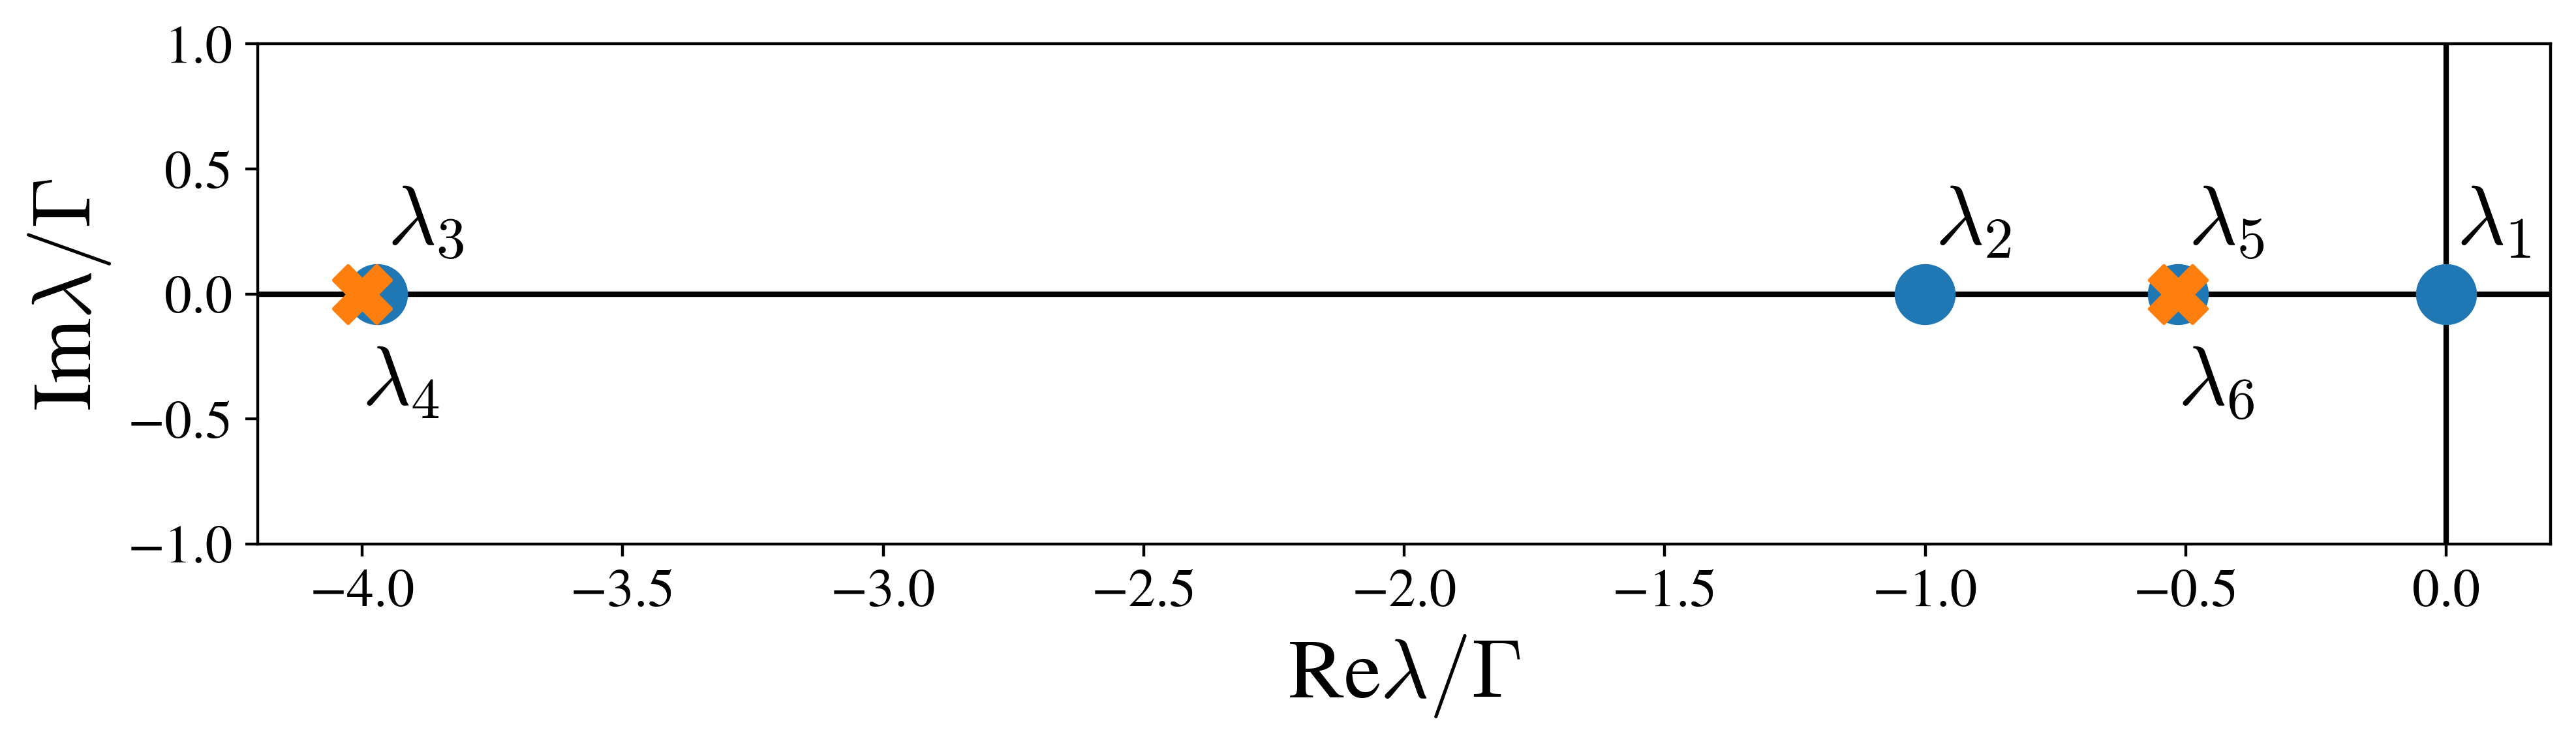
\includegraphics[width=0.8\linewidth]{figures/spectrum.png}
    \caption{The spectrum of the Liouvillian at the EP, where the degeneracy between $\lambda_5$ and $\lambda_6$ is the relevant one. The crosses are used to distinguish eigenvalues which are close to each other.}
    \label{fig:spec}
\end{figure}

\section{Dynamics}

Using \cref{eq:genmode}, the time evolution of the system can be given in terms of the eigenvalues and generalized eigenvectors of $L$. Away from an EP, the Liouvillian is diagonalizable, and the terms are purely exponential. The time evolution of the density operator is then given by
\begin{equation}\label{eq:dynnonep}
    \ket{\rho(t)}\rangle = \ket{\rho_{ss}}\rangle + \sum_{i=2}^6 c_i e^{\lambda_i t} \ket{\rho_i}\rangle,
\end{equation}
where $\ket{\rho_i}\rangle$ is the $i$th right eigenvector of $L$, and $c_i = \langle\braket{\sigma_i|\rho(0)}\rangle$. Here, $\langle\bra{\sigma_i}$ is the $i$th left eigenvector, constructed biorthogonally to $\ket{\rho_i}\rangle$ such that $\langle\braket{\sigma_i|\rho_j}\rangle = \delta_{ij}$, and $\ket{\rho_{ss}}\rangle = c_1 \ket{\rho_1}\rangle$ is the steady-state of the system. Furthermore, $\ket{\rho_{ss}}\rangle$ is the only eigenvector for which the first four elements add up to one, i.e., the only eigenvector which represents a density matrix with unity trace, see \cref{eq:order}. This implies that the rest of the other eigenvectors must be traceless for $\ket{\rho}\rangle$ to have unity trace. Hence, the eigenvectors $\ket{\rho_{i>1}}\rangle$, do not describe physical states on their own.

At the EP, the Jordan form of $L$ and its exponential, $\exp{(Jt)}$, have to be evaluated. Since the EP is of order two, this results in a $2\times2$ Jordan block. This is the only EP, which means that rest of the Jordan form is diagonal. Using \cref{eq:jordan,eq:expjordan}, this results in the following Jordan form and Jordan exponential:

\begin{equation}
    J = \begin{bmatrix} 0 & 0 & 0 & 0 & 0 & 0 \\
                        0 & \lambda_2 & 0 & 0 & 0 & 0 \\
                        0 & 0 & \lambda_3 & 0 & 0 & 0 \\
                        0 & 0 & 0 & \lambda_4 & 0 & 0 \\
                        0 & 0 & 0 & 0 & \bar \lambda & 1 \\
                        0 & 0 & 0 & 0 & 0 & \bar \lambda \\ \end{bmatrix}, \; 
        e^{Jt} = \begin{bmatrix} 1 & 0 & 0 & 0 & 0 & 0 \\
            0 & e^{\lambda_2t} & 0 & 0 & 0 & 0 \\
            0 & 0 & e^{\lambda_3t} & 0 & 0 & 0 \\
            0 & 0 & 0 & e^{\lambda_4t} & 0 & 0 \\
            0 & 0 & 0 & 0 & e^{\bar \lambda t} & t \\
        0 & 0 & 0 & 0 & 0 & e^{\bar \lambda t} \\ \end{bmatrix},
\end{equation}
since $\lambda_1 = 0$.

Furthermore, the Jordan chain vector, here written as $\ket{\rho'}\rangle$, defined by
\begin{equation}
    (L - \bar\lambda I)\ket{\rho'}\rangle = \ket{\bar\rho}\rangle,
\end{equation}
and the left generalized eigenvectors $\langle\bra{\sigma'}$ and $\langle\bra{\bar\sigma}$, need to be evaluated. The left generalized eigenvectors are constructed such that $\langle\braket{\sigma'|\rho'}\rangle = \langle\braket{\bar\sigma|\bar\rho}\rangle = 1$, and orthogonal to all other right generalized eigenvectors. Inserting these vectors into \cref{eq:genmode} leads, after a bit of work, to
\begin{equation}\label{eq:dynep}
    \begin{aligned}
        \ket{\rho(t)}\rangle = \ket{\rho_{ss}}\rangle + \sum_{i=2}^4 c_i e^{\lambda_i t} \ket{\rho_i}\rangle  
                                + (\bar c + c't)e^{\bar \lambda t}\ket{\bar \rho}\rangle + c'e^{\bar\lambda t}\ket{\rho'}\rangle,
    \end{aligned}
\end{equation}
where $\bar c = \langle\braket{\bar\sigma|\rho(0)}\rangle$, and $c' = \langle\braket{\sigma'|\rho(0)}\rangle$.

By numerically calculating the generalized eigenvectors as described in \cref{sec:jordan}, the dynamics at and away from the EP, given by \cref{eq:dynnonep,eq:dynep}, were implemented. The results were then compared with a numerical ODE-solver. The numerical solver was set to an absolute and relative tolerance of $10^{-10}$ and $10^{-6}$ respectively. The relative difference from the implemented methods to the numerical solver, given by $||\rho(t) - \rho_\text{num}(t)||_1/||\rho_\text{num}(t)||_1$, was in the order of $10^{-8}$ at all times, at and away from the EP. Here, $||\cdot||_1$ represents the matrix 1-norm, i.e. the maximum absolute column sum of the matrix. With the use of strict tolerances of the numerical solver, the small relative difference indicates an accurate method. Furthermore, when reducing the tolerances even more, the distance kept lowering, indicating that the numerical solver might be the limiting factor. It is hence clear that the implemented methods produce an accurate result at and away from the EP. 

%see \cref{fig:minevsint}.

% \begin{figure}[H]
%     \centering
%     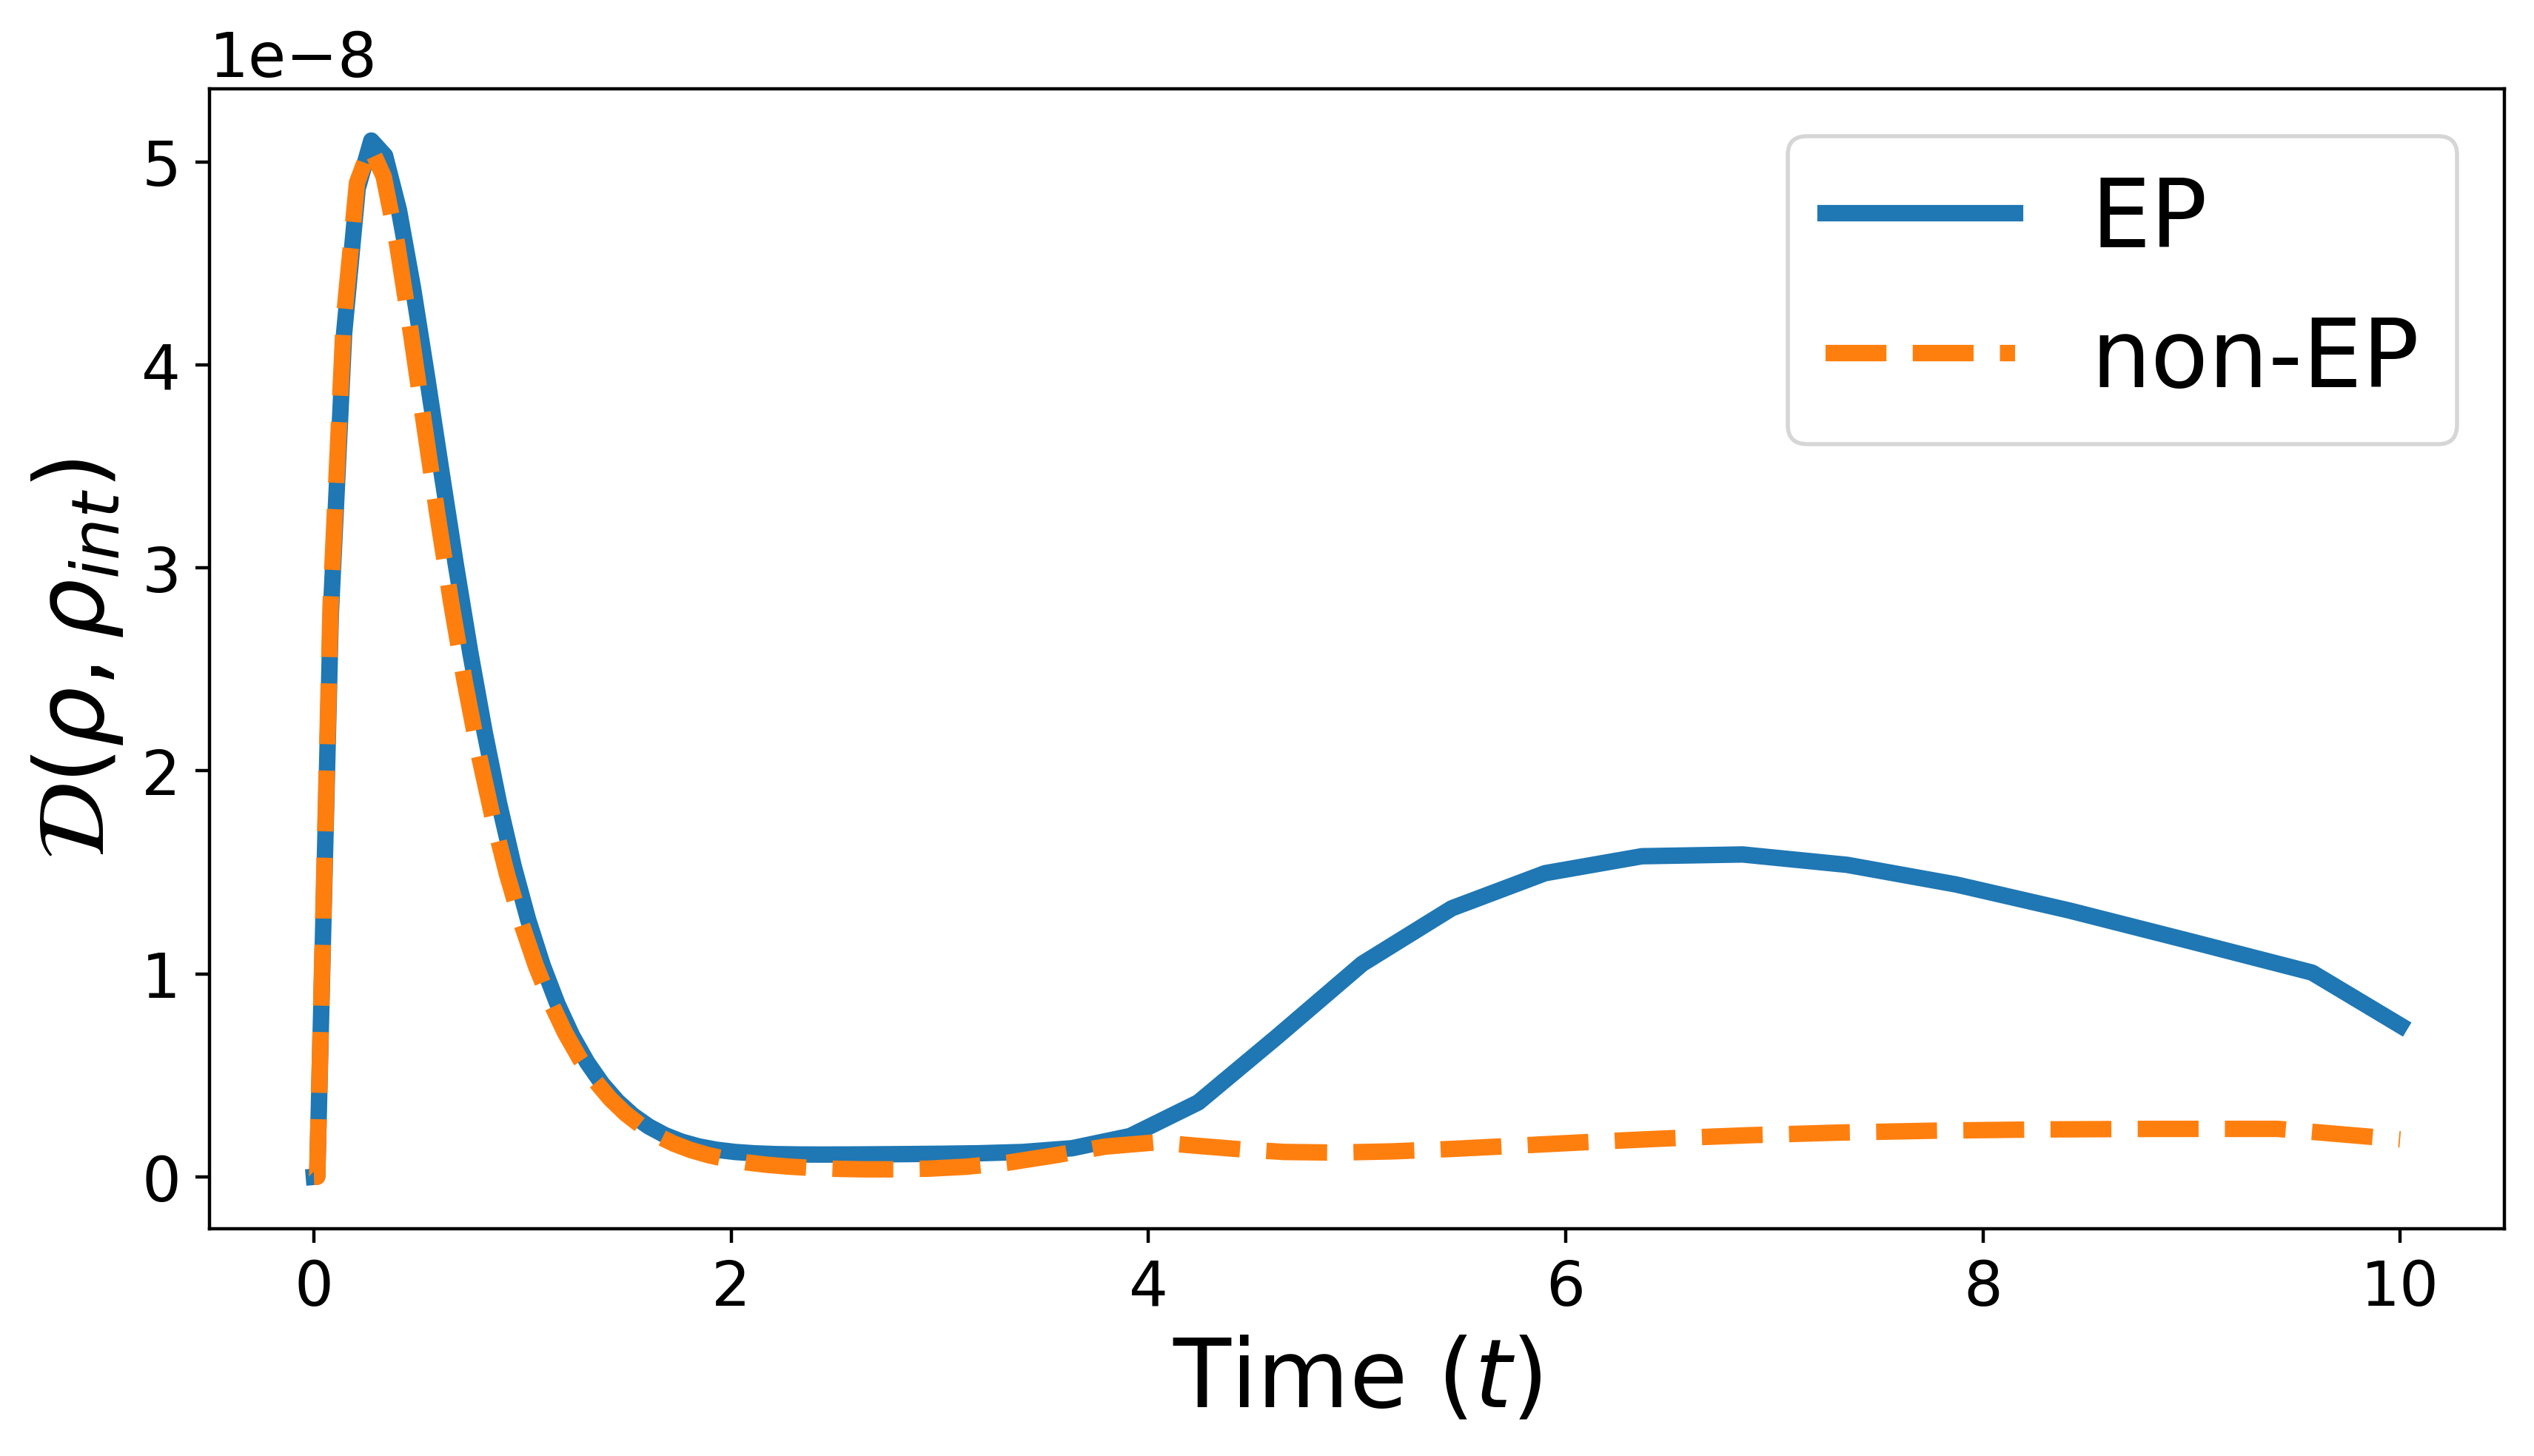
\includegraphics[width=0.6\linewidth]{figures/minevsint.png}
%     \caption{The relative difference $\mathcal{D}(\rho, \rho_\text{int}) = ||\rho - \rho_\text{int}||_1/||\rho_\text{int}||_1$ between the density matrices calculated with the implemented methods and with a numerical solver. The two lines represent the distances at the EP and away from the EP, using the corresponding implemented methods for each case. The numerical solver was set to an absolute and relative tolerance of $10^{-10}$ and $10^{-6}$ respectively.}
%     \label{fig:minevsint}
% \end{figure}

\subsection{Varying initial conditions}

With a clear picture of the analytical dynamics and numerically calculated eigenvalues and generalized eigenvectors at hand, simulations of the parallel dot system were performed. Firstly, the time evolution in the generalized modes was investigated. This was done by introducing initial conditions consisting of linear combinations of the generalized eigenvectors
\begin{equation}\label{eq:ini}
    \ket{\rho(0)}\rangle = \ket{\rho_{ss}}\rangle + \sum_{i=2}^4 b_i\ket{\rho_i}\rangle + \bar b \ket{\bar\rho}\rangle + b'\ket{\rho'}\rangle.
\end{equation}
This way, the constants $c$ in \cref{eq:dynep} are the same as the corresponding constants labeled with $b$ in \cref{eq:ini}. The generalized modes included in the time evolution can then be controlled by the initial condition. To see this, simulations of the density matrix for different initial conditions were done and then compared with the steady-state of the system, see \cref{fig:rhodiffrho0}. 
\begin{figure}[H]
\centering
\begin{subfigure}[t]{.5\textwidth}
  \centering
  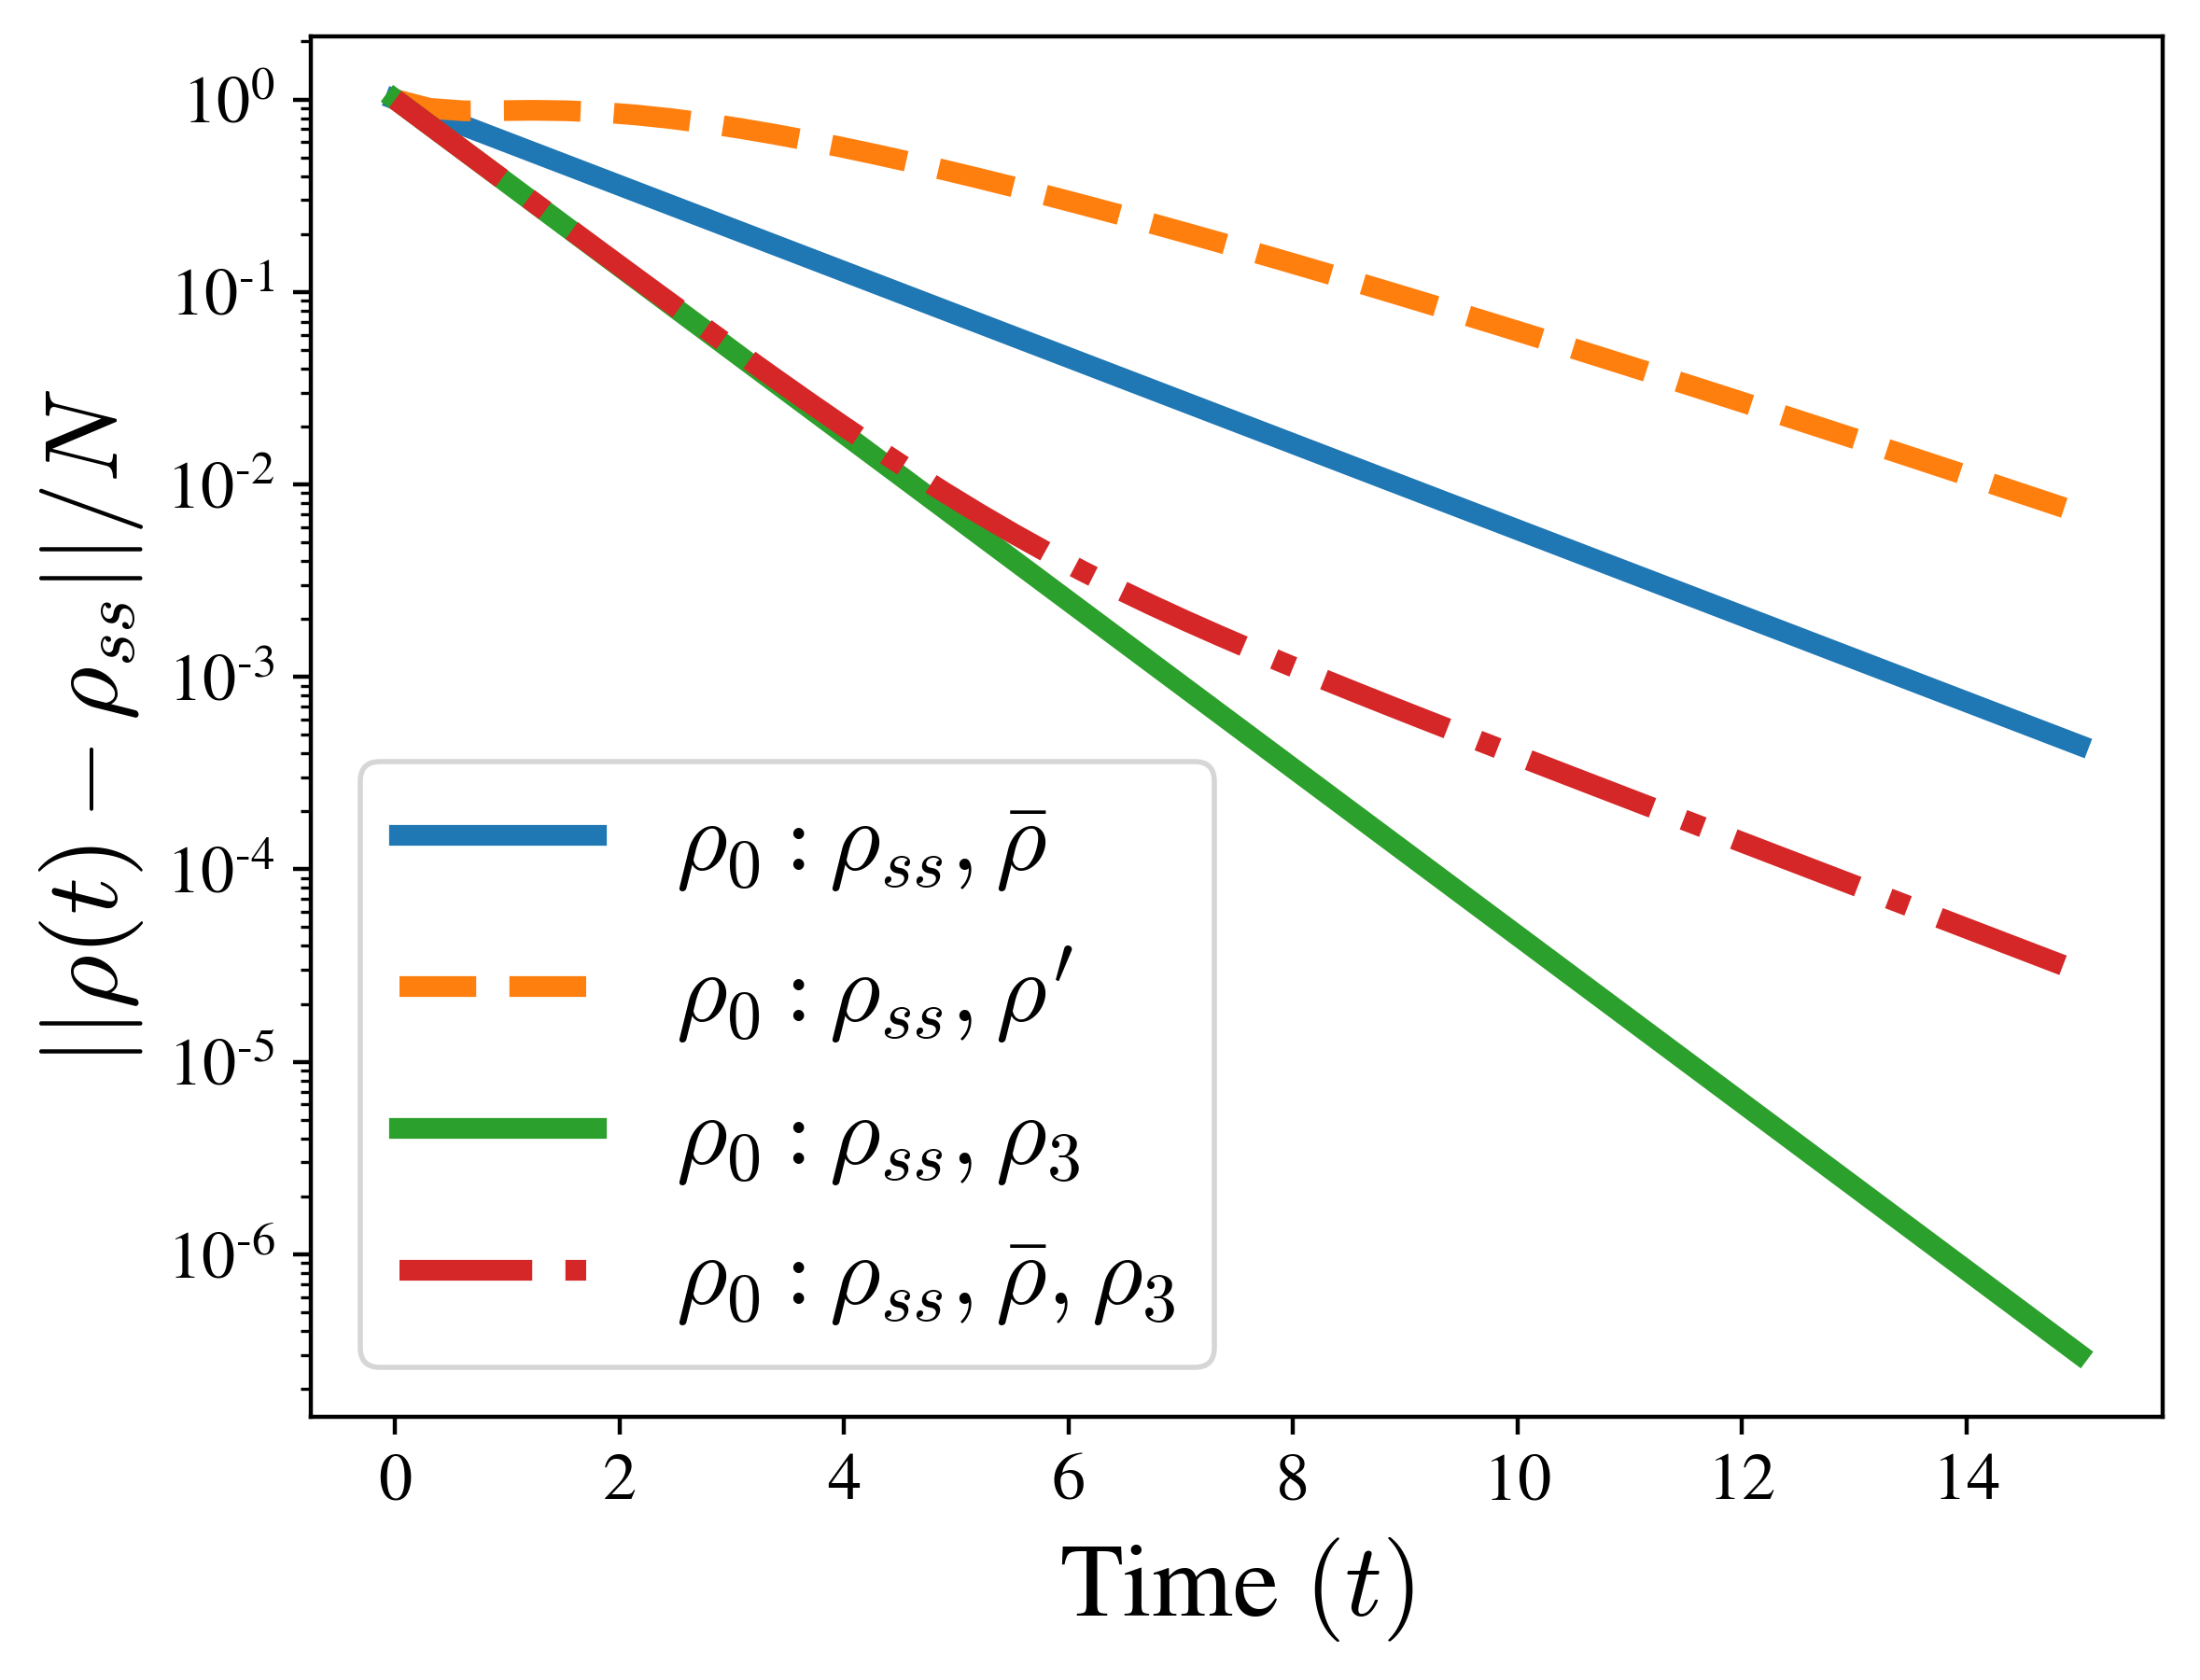
\includegraphics[width=\linewidth]{figures/rho_diff_rho0_v4.png}
  \caption{}
  \label{fig:rhodiffrho0}
\end{subfigure}%
\begin{subfigure}[t]{.5\textwidth}
  \centering
  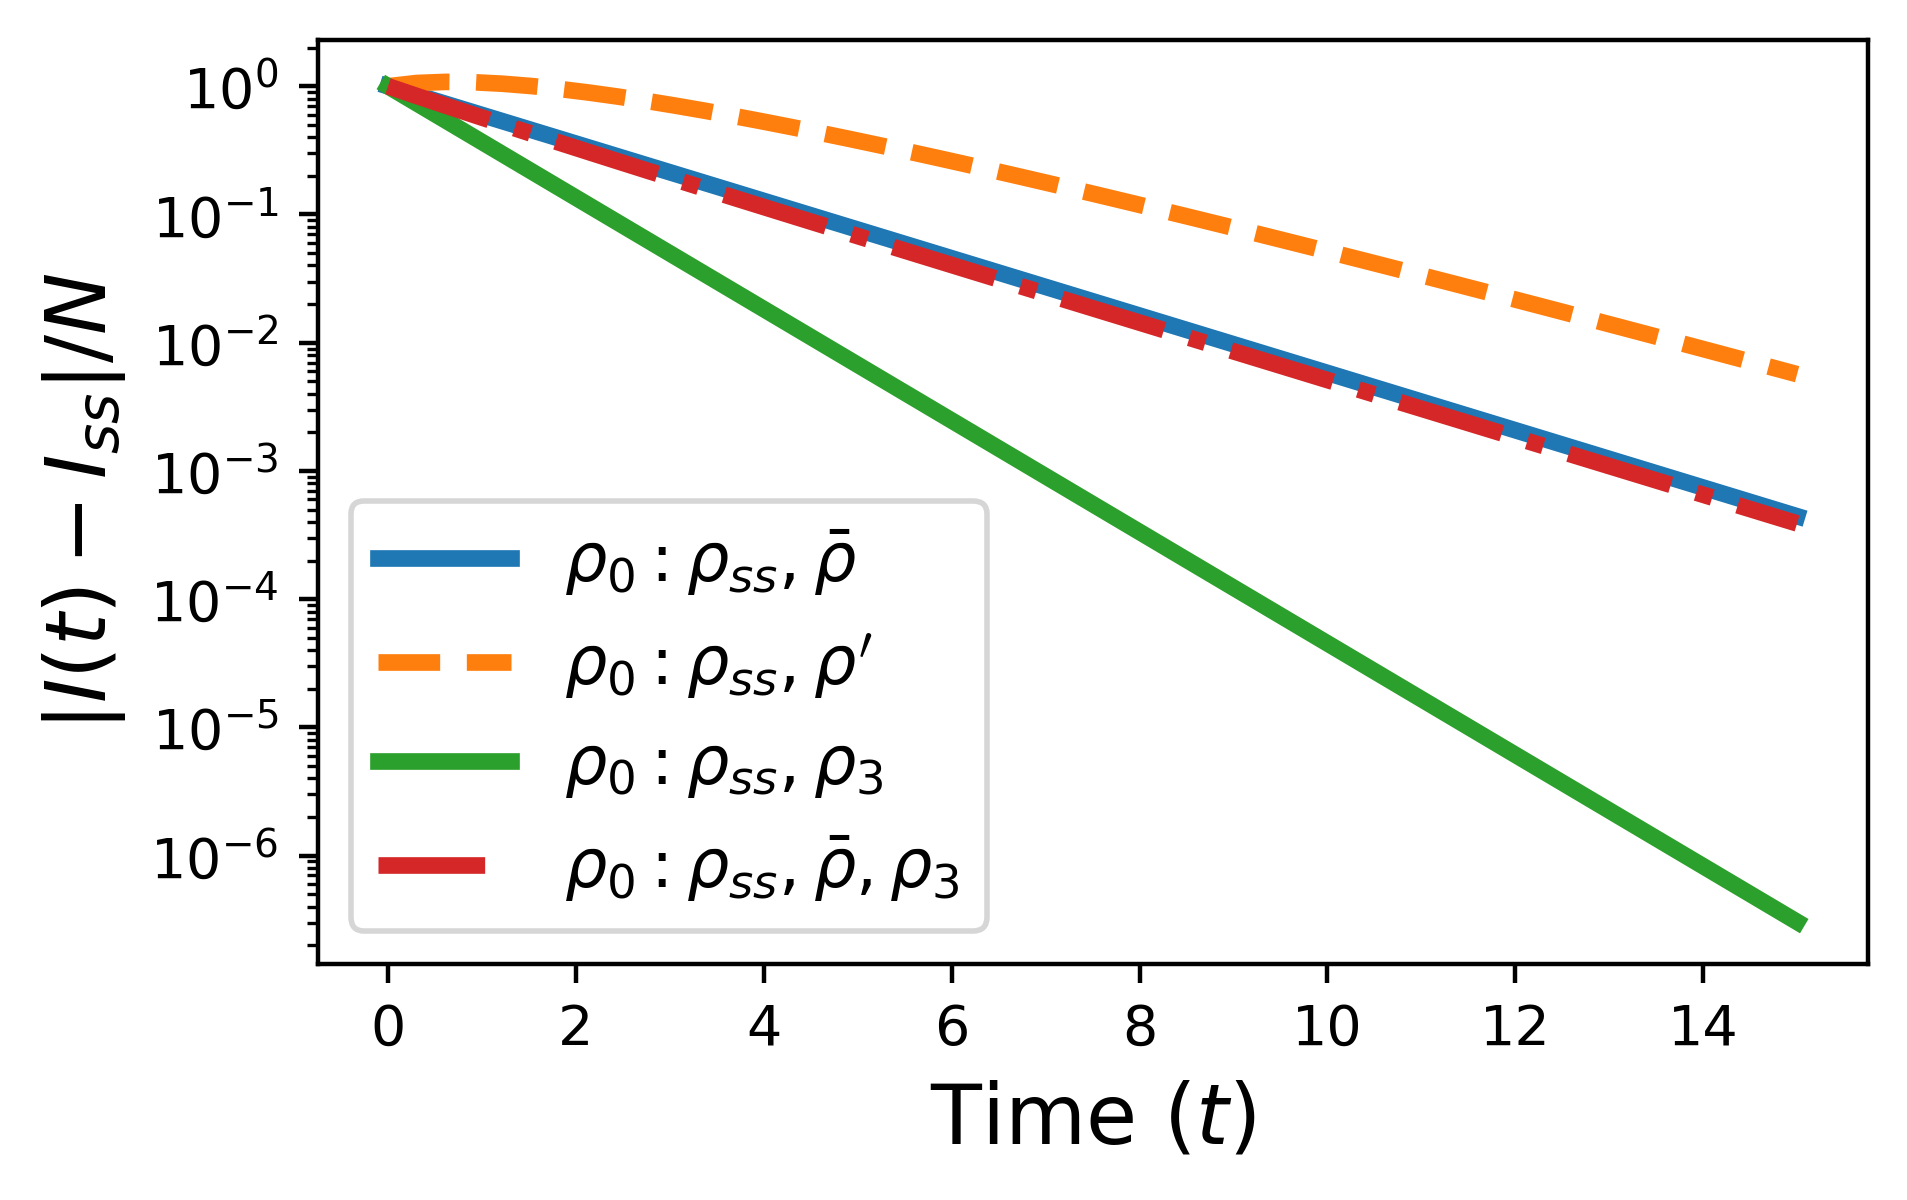
\includegraphics[width=\linewidth]{figures/I_diff_rho0_nonvis.png}
  \caption{}
  \label{fig:Idiffrho0}
\end{subfigure}
\caption{The decay of the density matrix (a) and the current (b), towards the steady-state density matrix $\rho_{ss}$ and current $I_{ss}$ in a logarithmic plot. The simulations were done at the EP with different initial conditions in linear combinations of the generalized eigenvectors, see \cref{eq:ini}. The linear combinations used for the initial conditions are given by the following: the solid, blue line: $\bar b = 1$, the dashed, yellow line: $b'=1$, the solid, green line: $b_3=1$, and the dash-dotted, red line: $\bar b=1,$ \\{$b_3=15$}, all other constants being zero if not mentioned. A normalization by \\{$N=||\rho(0) - \rho_{ss}||$} and $N=|I(0) - I_{ss}|$ was done such that each curve is unity for $t=0$. Here, $||\cdot||$ represents the Euclidean norm of the vectorized density matrices.}
\label{fig:diffrho}
\end{figure}

% \begin{table}[H]
%     \centering
%     \caption{The initial conditions used for the simulations in \cref{fig:diffrho}, in terms of the constants labeled $b$ in \cref{eq:ini}. Only the non-zero constants are included in the table.}
%     \begin{tabular}{c|c}\label{table:tab}
%         Line & Constants \\\hline 
%         Solid, blue & $\bar b = 1$ \\
%         Dashed, yellow & $b'=1$ \\
%         Solid, green & $b_3 = 1$ \\
%         Dash-dotted, red & $\bar b = 1, b_3 = 15$ \\
%     \end{tabular}
% \end{table}
With initial conditions including only one $b_i\neq0$ or $\bar b\neq0$, i.e., only one normal eigenvector excluding $\ket{\rho_{ss}}\rangle$, a mode consisting of pure exponential decay toward the steady-state is seen by the straight lines in the logarithmic plot. This is expected since the time evolution only picks up one of the exponentials from \cref{eq:dynep}. The quicker decay corresponds to $\ket{\rho_3}\rangle$ since $|\lambda_3| > |\bar\lambda|$, see \cref{fig:spec}. When including both $\ket{\bar \rho}\rangle$ and $\ket{\rho_3}\rangle$ in the initial condition, the decay first follows the quicker decay channel, then gradually turns into following the decay of $\ket{\bar\rho}\rangle$. Another behavior is seen for the initial condition including $\ket{\rho'}\rangle$. This generalized mode is not of exponential nature, since a factor of $t\exp(\bar\lambda t)$ enters in the dynamics. Away from an EP, the dynamics is given by \cref{eq:dynnonep} and this type of algebraic decay never happens. Thus, the behavior of this decay channel is a unique feature of the EP dynamics.

As discussed in \cref{sec:theory}, any relevant observable of the system can be obtained from the density operator. For the parallel dot system, the main observable is the current entering or leaving a lead, which by using \cref{eq:expec} can be obtained by
\begin{equation}\label{eq:current}
    \braket{\hat I_s}(t) = \tr{(\hat \rho(t)\hat I_s)},
\end{equation}
with a current operator $\hat I_s$, corresponding to the current out of lead $s\in\{\text{L,R}\}$. The current operators can be phrased in terms of the jump operators from the Lindblad equation as 
\begin{equation}\label{eq:currjump}
    \hat I_s = \hat J_{s+}^\dag \hat J_{s+} - \hat J_{s-}^\dag \hat J_{s-},
\end{equation}
where $\hat J_{s\alpha}$, $\alpha\in\{+,-\}$, is the jump operator corresponding to tunneling events entering (+) a dot from lead $s$ or leaving (-) a dot to lead $s$.

By calculating and collecting the jump operators using the aforementioned code implementing the PERLind approach and then inserting \cref{eq:currjump} into \cref{eq:current}, the current through the QD system could be simulated. In \cref{fig:Idiffrho0}, the calculations from \cref{fig:rhodiffrho0} were used to also simulate the current for the same initial conditions. The results are similar to the simulations of the density matrix, indicating that the time evolution in generalized modes carry over to the transient current dynamics. However, with the initial condition including the two normal eigenvectors, the decay in the quicker decay channel is washed out in this time scale and seemingly only follows the slower decay rate. This can be contrasted with the algebraic decay, which is equally visible in the current dynamics as in the density matrix dynamics.

% \begin{equation}
%     \hat{I}_s(t) = \diff{}{t}\hat{N}_s(t) = -i [\hat H, \hat{N}_s(t)],
% \end{equation}

\subsection{Varying parameters}

Simulations were also done to investigate the general behavior of the current at and slightly away from the EP. This is done in \cref{fig:diffI}, for two different initial conditions: one with empty dots, and the other in a mixed state. These initial vectorized density matrices are given by
% \begin{equation}\label{eq:initialI}
% \begin{split}
%     1: \rho(0) = \rho_\text{empty} = &\begin{bmatrix} 1 & 0 & 0 & 0 \\
%                                              0 & 0 & 0 & 0 \\
%                                              0 & 0 & 0 & 0 \\
%                                          0 & 0 & 0 & 0 \end{bmatrix},\\ \\
%         2: \rho(0) = \rho_\text{mixed} = 1/4 &\begin{bmatrix} 1 & 0 & 0 & 0 \\
%                                              0 & 1 & 0 & 0 \\
%                                              0 & 0 & 1 & 0 \\
%                                             0 & 0 & 0 & 1 \end{bmatrix}.
% \end{split}
% \end{equation}
\begin{equation}\label{eq:initialI}
\begin{split}
    1: \ket{\rho(0)}\rangle &= \ket{\rho_\text{empty}}\rangle = \begin{bmatrix} 1 & 0 & 0 & 0 & 0 & 0 \end{bmatrix}^T\\
    2: \ket{\rho(0)}\rangle &= \ket{\rho_\text{mixed}}\rangle = \frac{1}{4}\begin{bmatrix} 1 & 1 & 1 & 1 & 0 & 0\end{bmatrix}^T.
\end{split}
\end{equation}

\begin{figure}[H]
\centering
\begin{subfigure}[t]{.5\textwidth}
  \centering
  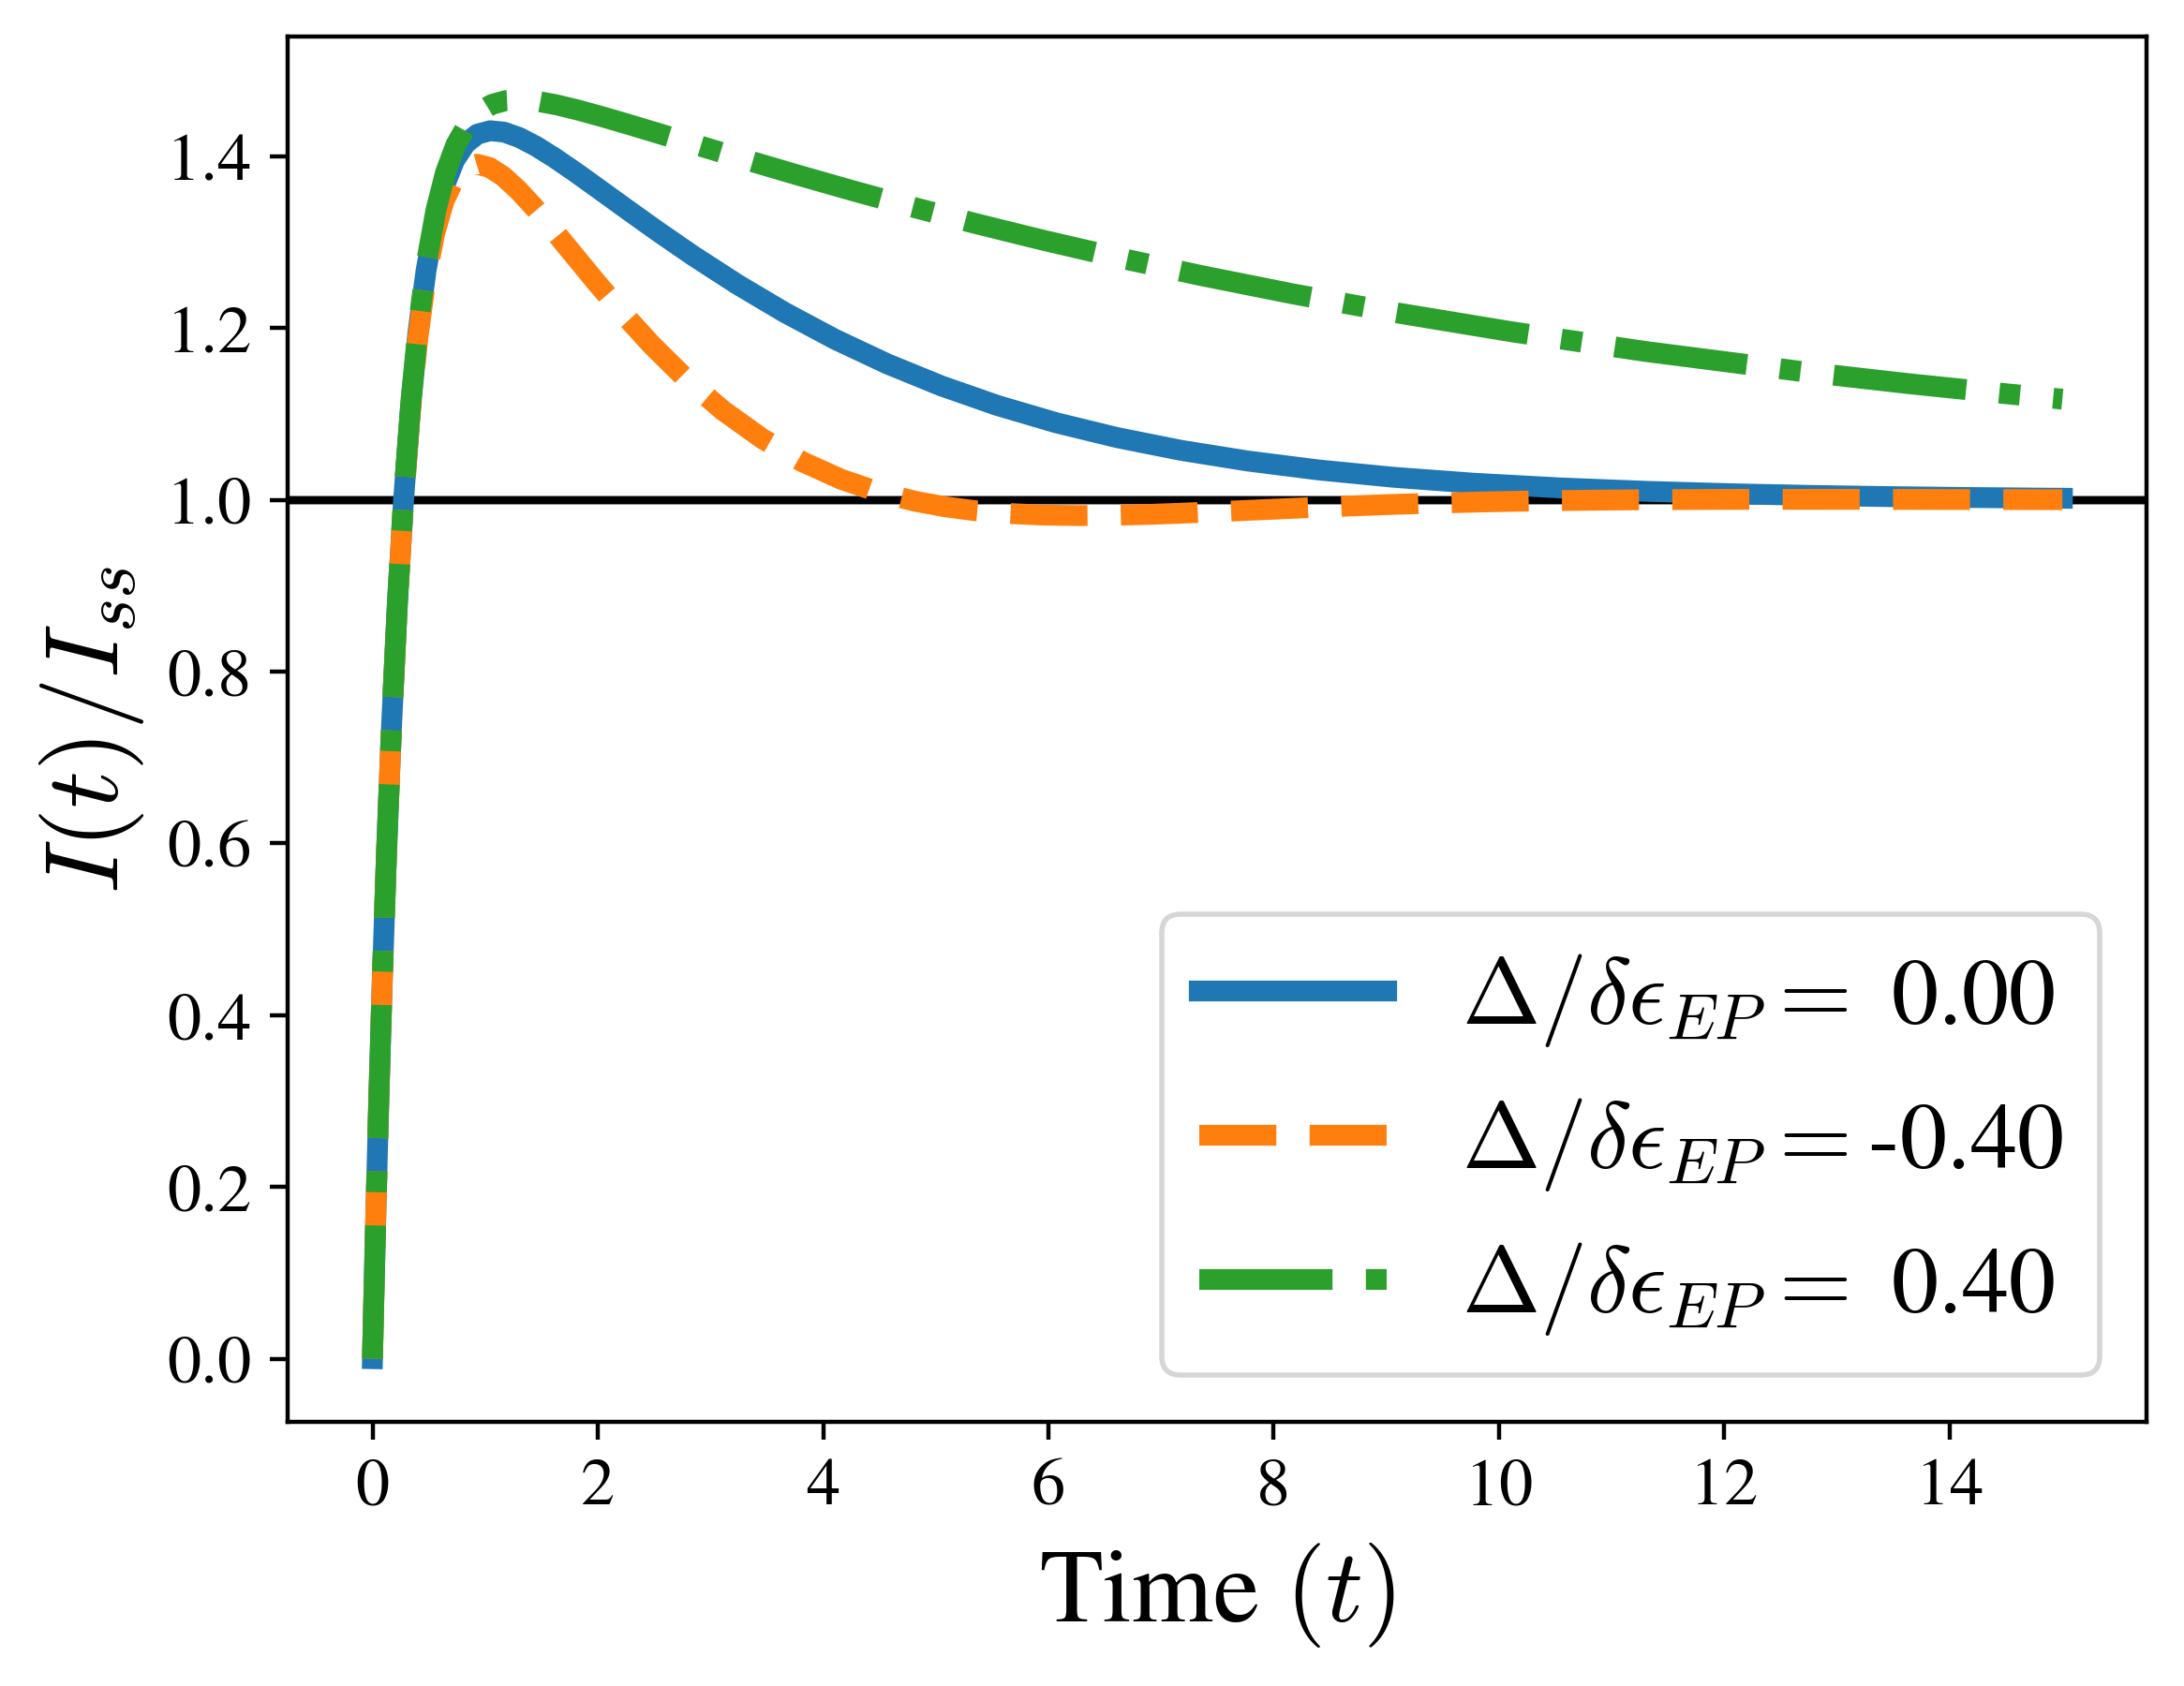
\includegraphics[width=\linewidth]{figures/diffde_empty.png}
  \caption{}
  \label{fig:diffde1}
\end{subfigure}%
\begin{subfigure}[t]{.5\textwidth}
  \centering
  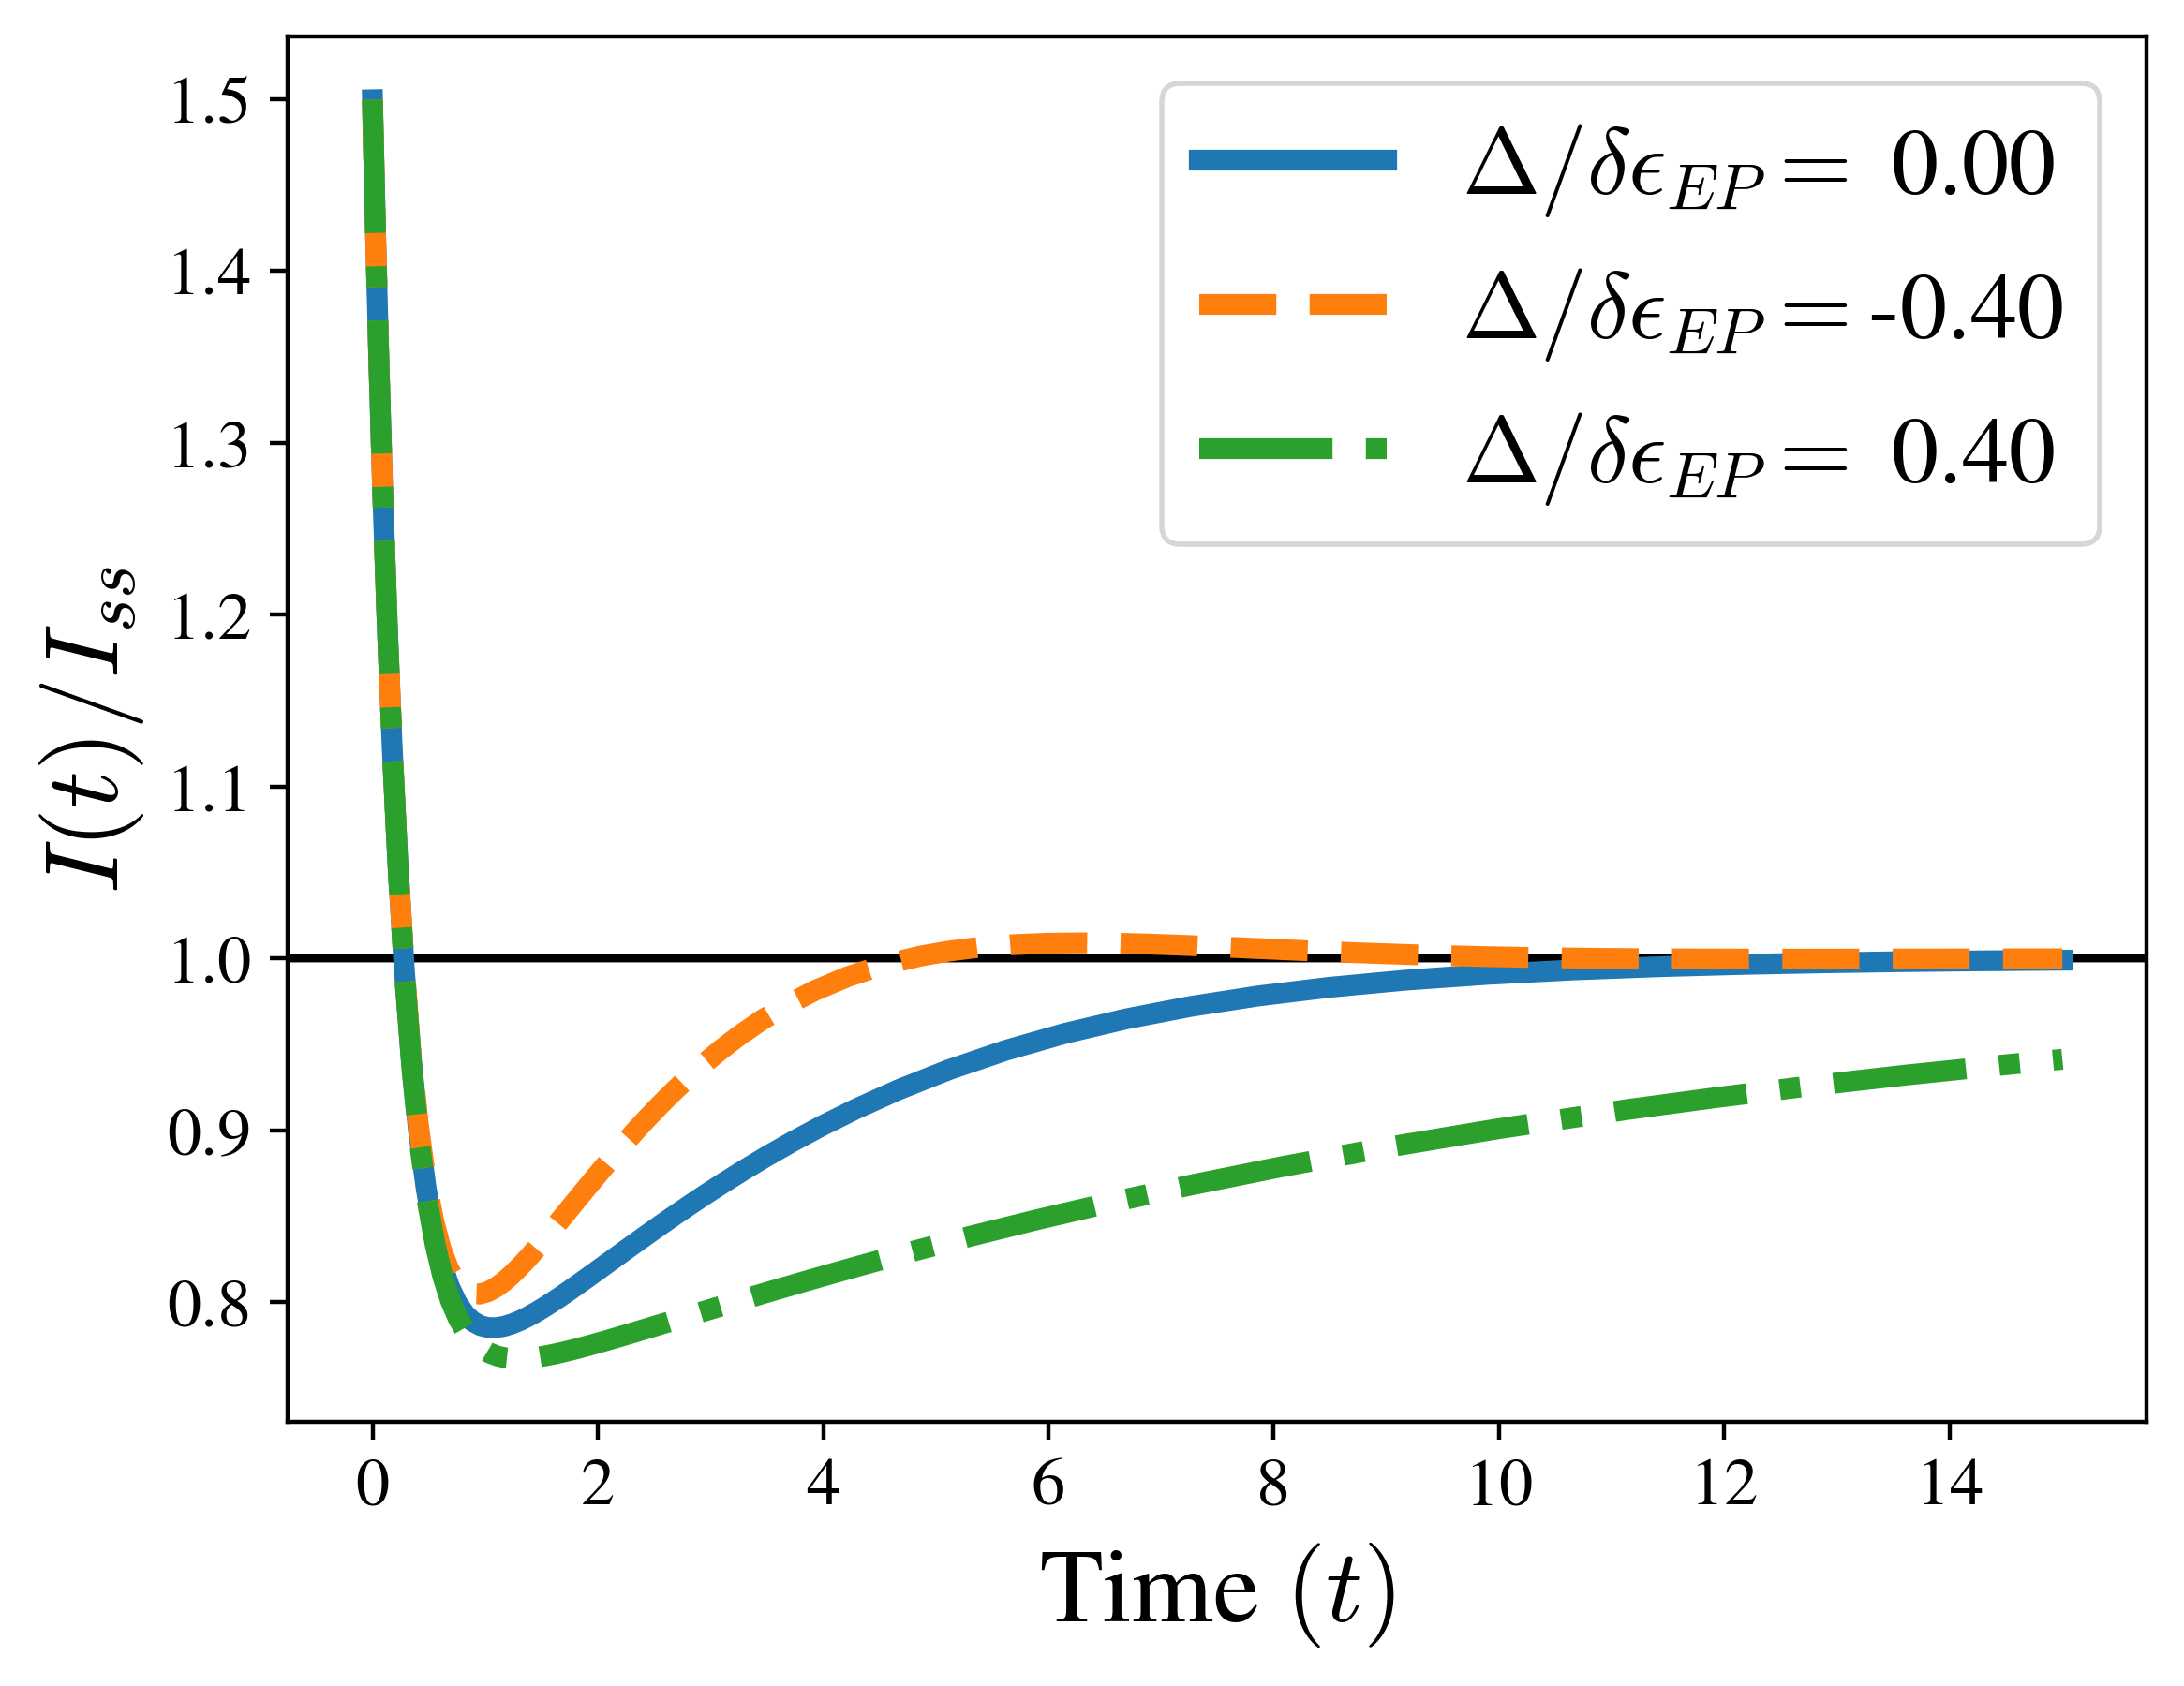
\includegraphics[width=\linewidth]{figures/diffde_mixed.png}
  \caption{}
  \label{fig:diffde2}
\end{subfigure}
\caption{The current over time for different $\Delta = \delta\epsilon_\text{EP} - \delta\epsilon$, normalized by the corresponding steady-state current $I_{ss}$. The solid, blue curves correspond to the system being at the EP, while the other two are slightly away from it. The initial conditions are given by \cref{eq:initialI}, with a) having the empty initial condition and b) the mixed one.}
\label{fig:diffI}
\end{figure}
Looking at \cref{fig:diffI}, it is clear that the three curves behave differently after the first phase of overshooting the steady-state, i.e., after $t\approx 2$. The curves corresponding to a $\Delta<0$, slightly overshoot the steady-state once more before approaching the steady-state solution. This can be phrased as an underdamped behavior. On the other hand, for $\Delta>0$, the decay towards the steady-state is very slow, which can be thought of as an overdamped system. Lastly, for the system at the EP, the decay is much faster than for the overdamped system, but does not overshoot the steady-state again like the underdamped system. This behavior is similar to what was found in Ref.~\cite{thermal} for quantum thermal machines, where the dynamics at the EP corresponded to the quickest decay without overshooting the steady-state, which is known as critical damping. Furthermore, it can be noted that the current dynamics in \cref{fig:diffI} varies continuously when approaching and leaving the EP, even though the notion of EPs at first sight does seem to invoke abrupt changes.
\end{document}
